%! Licence = CC BY-NC-SA 4.0

%! Author = gianfluetsch
%! Date = 19. Jan 2022
%! Project = pfsec_summary

\section{Operating System Security}

\subsection{Introduction}

\subsubsection{Layers}
\textit{User Applications and Utilities $\rightarrow$ Operating System Kernel $\rightarrow$ Physical Hardware}\\

Das Vorhandensein von BIOS und möglicherweise anderem Code, der außerhalb des Betriebssystemkerns liegt und Betriebssystem-Kernel nicht sichtbar ist, aber beim Booten des Systems verwendet wird des Systems oder zur Unterstützung der Low-Level-Hardware-Steuerung verwendet wird, ist in den Schichten.
Für jede dieser Layer müssen geeignete Hardening-Massnahmen ergriffen werden um angemessene Sicherheitsdienste bereitzustellen. Und jeder Layer ist anfällig für Angriffe von unten angreifbar, wenn die unteren Schichten nicht auch entsprechend gesichert sind.

\subsubsection{Strategies}
\begin{enumerate}
    \item White-list approved applications
    \begin{itemize}
        \item Was (welche Applikation) darf auf welchem Layer laufen $\rightarrow$ Whitelisting
    \end{itemize}
    \item Patch third-party applications and operating system vulnerabilities
    \begin{itemize}
        \item Wann wird welcher Patch eingespielt, anhand möglicher Probleme etc. Strategie erstellen und umsetzen
    \end{itemize}
    \item Restrict administrative privileges
    \begin{itemize}
        \item Wirklich nur wenn nötig admin-Rechte vergeben oder Zeitbeschränkt admin-Rechte einrichten $\rightarrow$ Principle of Least Privileges
    \end{itemize}
    \item Create a defense-in-depth system
\end{enumerate}

\subsubsection{Build and Deploy Process}
\begin{itemize}
    \item Requirements on the build and deploy process:
    \begin{itemize}
        \item Assess risks and plan the system deployment
        \item Secure the underlying operating system and then the key applications
        \item Ensure any critical content is secured
        \item Ensure appropriate network protection mechanisms are used
        \item Ensure appropriate processes are used to maintain security
    \end{itemize}
    \item Note that the \textbf{system can already be compromised during the installation process} before it can install the latest patches.
\end{itemize}

\subsubsection{System Security Planning}
The aim of the specific system installation planning process is to maximize security while minimizing costs. Wide experience shows that it is much more
difficult and expensive to “retro-fit” security at a later time, than it is to plan and provide it during the initial deployment process.\\

The first step in deploying a new system is planning. Planning should include
\begin{itemize}
    \item a wide security assessment of the organization
    \item Aim is to maximize security while minimizing costs
    \item Planning process needs to determine security requirements for the system, applications, data, and users
    \item Plan needs to identify appropriate personnel and training to install and manage the system
    \begin{itemize}
        \item Tools like Splunk \& ElasticSearch\\
    \end{itemize}
\end{itemize}

\begin{center}
    \vspace{-8pt}
    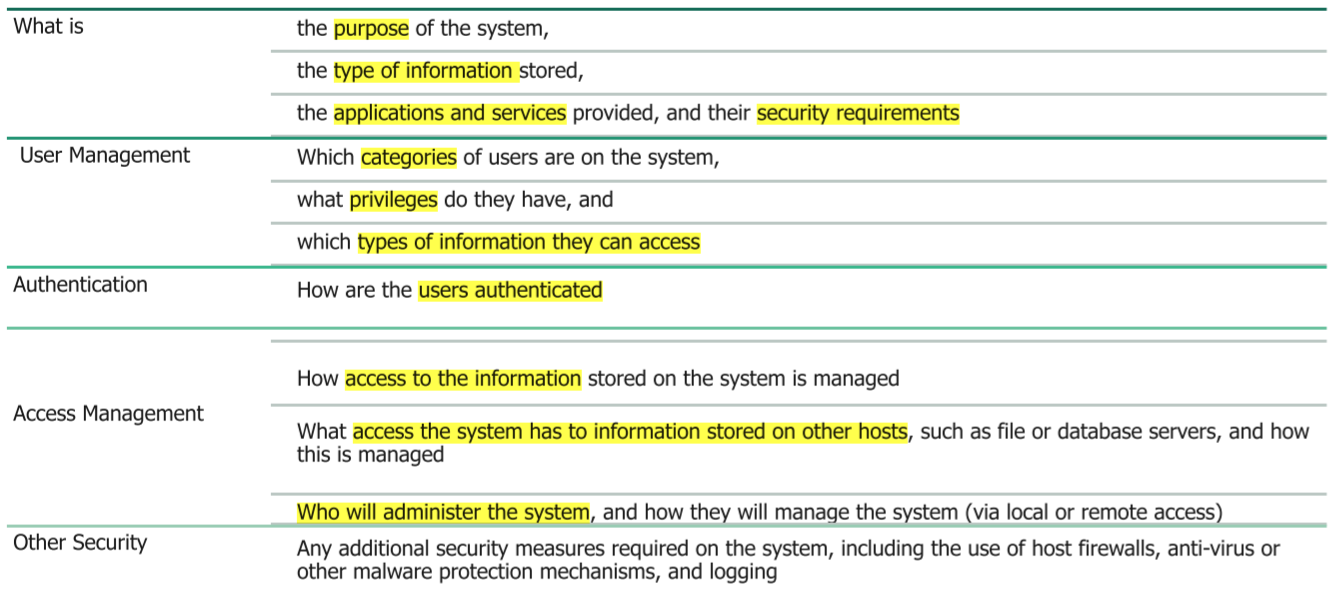
\includegraphics[width=1.0\linewidth]{03-operating_system_security/system_security_planning}
    \vspace{-8pt}
\end{center}

\subsection{OS Hardening}\label{subsec:os-hardening}

\subsubsection{Steps in OS Hardening}
\begin{enumerate}
    \item Install and patch the operating system
    \item Harden and configure the operating system to adequately address the identified security needs of the system by:
    \begin{itemize}
        \item Removing unnecessary services, applications, and protocols
        \item Configuring users, groups, and permissions
        \item Configuring resource controls
    \end{itemize}
    \item Install and configure additional security controls, such as anti-virus, host-based firewalls, and intrusion detection system (IDS)
    \item Test the security of the basic operating system to ensure that the steps taken adequately address its security needs
    \begin{itemize}
        \item Ensure the previous security configuration steps are correctly implemented \& identify possible vulnerabilities
        \item Review a system to ensure that a system meets the basic security requirements
        \item Scan for known vulnerabilities and poor configuration practices\\
    \end{itemize}
\end{enumerate}

\textcolor{red}{\textbf{Wenn zwischen Schritt 1 \& 2 schon jemand Zugriff auf das System hat und etwas schädliches einspielen könnte, kann man es gerade sein lassen $\rightarrow$ bereits kompromitiertes System.}}

\subsubsection{Application Configuration}
\begin{itemize}
    \item Creating and specifying appropriate data storage areas for application
    \item Making appropriate changes to the application or service default configuration details
    \begin{itemize}
        \item may include: default data, scripts or user accounts
    \end{itemize}
    \item Risk from remotely accessed services such as Web and file transfer services is reduced by ensuring that most of the files can only be read, but not written, by the server
\end{itemize}

\subsubsection{Encryption Technology}
\begin{itemize}
    \item Is a key enabling technology that may be used to secure data both in transit and when stored
    \item Must be configured and appropriate cryptographic keys created, signed, and secured
    \item If secure network services are provided using TLS or IPsec suitable public and private keys must be generated for each of them
    \item If secure network services are provided using SSH, appropriate server and client keys must be created
    \item Cryptographic file systems are another use of encryption
\end{itemize}

\subsubsection{Maintaining Security is continuous}
Security maintenance includes:
\begin{itemize}
    \item Monitoring and analyzing logging information
    \item Performing regular backups
    \item Recovering from security compromises
    \item Regularly testing system security
    \item Using appropriate software maintenance processes to patch and update all critical software, and to monitor and revise configuration as needed
\end{itemize}

\subsubsection{Logging as cornerstone}
\begin{itemize}
    \item Can only inform you about bad things that have already happened
    \item In the event of a system breach or failure, system administrators can more quickly identify what happened
    \item Key is to ensure you \textbf{capture the correct data} and then appropriately monitor and analyze this data
    \item Information can be generated by the system, network and applications
    \item Range of data acquired should be determined during the system planning stage
    \item Generates significant volumes of information and it is important that sufficient space is allocated for them
    \item Automated analysis is preferred
\end{itemize}

\subsubsection{Backup as another cornerstone}
\begin{center}
    \vspace{-8pt}
    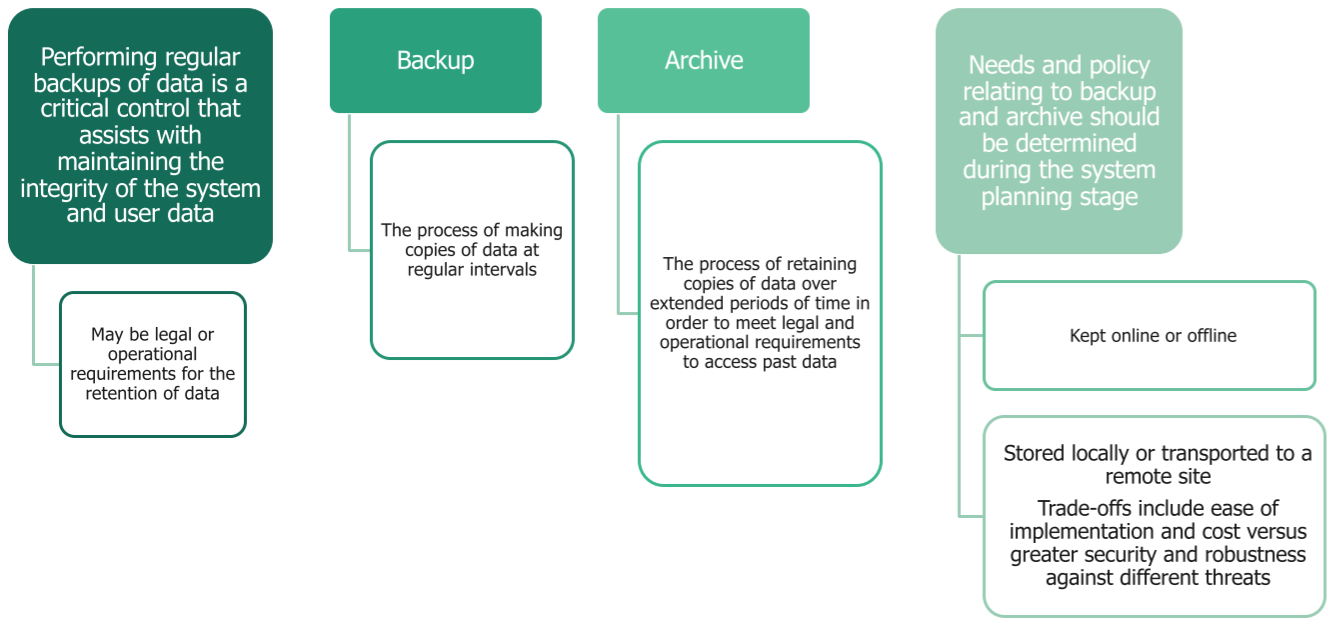
\includegraphics[width=1.0\linewidth]{03-operating_system_security/backup}
    \vspace{-8pt}
\end{center}

\subsection{Virtualization}

\subsubsection{Virtualization Security Issues}

\begin{minipage}{0.5\linewidth}
    \begin{itemize}
        \item \textbf{Guest OS isolation}
        \begin{itemize}
            \item Ensuring that programs executing within a guest OS may only access and use the resources allocated to it
        \end{itemize}
        \item \textbf{Guest OS monitoring by the hypervisor}
        \begin{itemize}
            \item Which has privileged access to the programs and data in each guest OS
        \end{itemize}
        \item \textbf{Virtualized environment security}
        \begin{itemize}
            \item Particularly image and snapshot management which attackers may attempt to view or modify
        \end{itemize}
    \end{itemize}
\end{minipage}
\begin{minipage}{0.45\linewidth}
    \begin{center}
        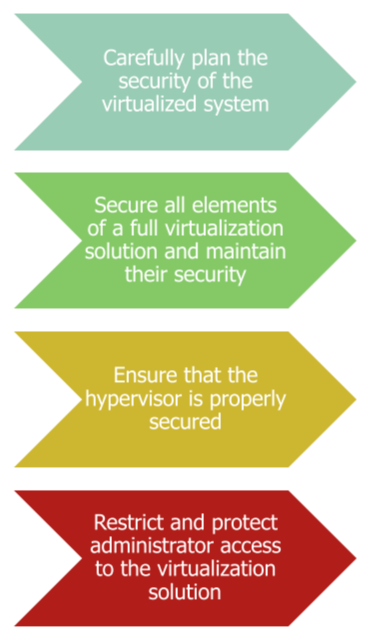
\includegraphics[width=0.4\linewidth]{03-operating_system_security/virtualization}
        \vspace{-8pt}
    \end{center}
\end{minipage}

\subsubsection{Hypervisor Security}
\begin{itemize}
    \item Should be Secured using a process similar to securing an operating system
    \item Installed in an isolated environment
    \item Configured so that it is updated automatically
    \item Monitored for any signs of compromise
    \item Accessed only by authorized administration
    \item May support both local and remote administration so must be configured appropriately
    \item Remote administration access should be considered and secured in the design of any network firewall and IDS capability in use
    \item Ideally administration traffic should use a separate network with very limited access provided from outside the organization
\end{itemize}

\subsubsection{Virtualizes Infrastructure Security}
\begin{itemize}
    \item Access to VM image and snapshots must be carefully controlled
    \item Access must be limited to just the appropriate guest OSs
    \item Systems manage access to hardware resources
\end{itemize}

\subsubsection{Virtual Firewall}
\begin{center}
    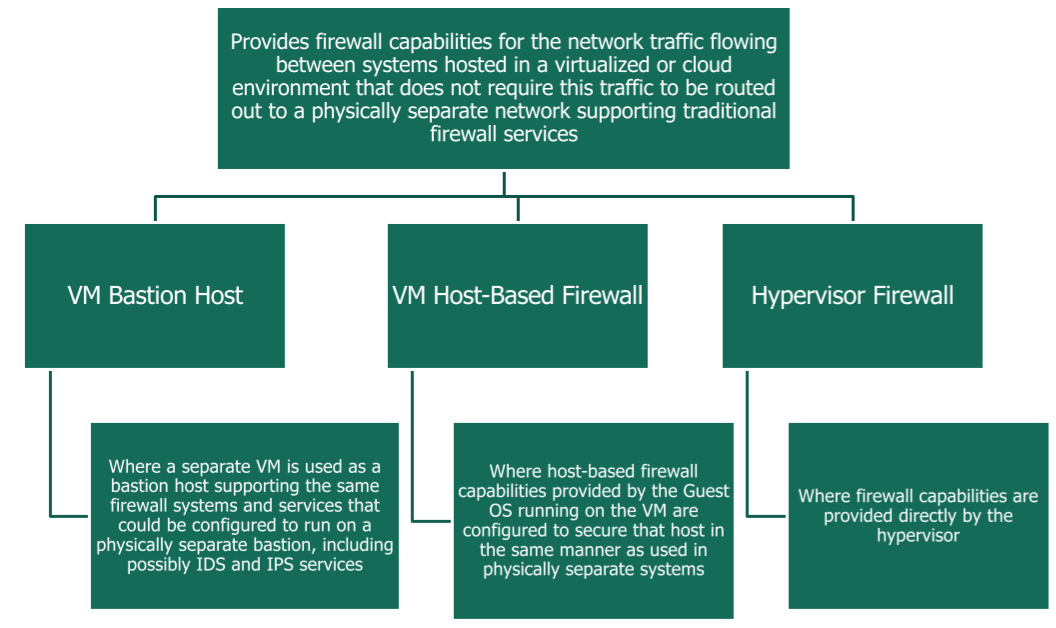
\includegraphics[width=.9\linewidth]{03-operating_system_security/virtual_fw}
    \vspace{-8pt}
\end{center}


